\documentclass[12pt, a4paper]{article}
\edef\restoreparindent{\parindent=\the\parindent\relax}
\usepackage{XCharter}
\usepackage[utf8]{inputenc}
\usepackage[T1]{fontenc}
\usepackage{amsmath}
\usepackage[UKenglish]{babel}
\usepackage[bibstyle=ieee, dashed=false, sorting=nty]{biblatex}
\usepackage[labelfont=bf]{caption}
\usepackage{csquotes}
\usepackage{fancyhdr}
\usepackage{float}
\usepackage[top=25mm, right=25mm, bottom=20mm, left=25mm]{geometry}
\usepackage{graphicx}
\usepackage[hidelinks]{hyperref}
\usepackage{listings}
\usepackage{adjustbox, makecell}
\usepackage{microtype}
\usepackage{multicol}
\usepackage{parskip}
\usepackage{titlesec}
\usepackage{xcolor}
\usepackage{xparse}

\restoreparindent

\pagestyle{fancy}
\fancyhead[L]{COM4506}
\fancyhead[C]{Assignment: Metamorphic Testing}
\fancyhead[R]{acb16zje}
\setlength{\headheight}{15pt}

\setcounter{secnumdepth}{4}

% \titleformat{\paragraph}
% {\normalfont\normalsize\bfseries}{Category \Alph{subsubsection}\arabic{paragraph}}{1em}{}
% \titlespacing*{\paragraph}{0pt}{3.25ex plus 1ex minus .2ex}{1.5ex plus .2ex}

% \newcounter{category}[subsubsection]
% \newcommand{\category}[2]{\stepcounter{category} \textbf{Category #1\thecategory: #2} \par}

\newcounter{category}[subsection]
\newenvironment{category}[3][]{\refstepcounter{category}\par\medskip
\noindent \underline{\textbf{Category~#1\thecategory \quad #2}} \rmfamily\par #3}{\medskip}

\renewcommand{\arraystretch}{1.3}

\definecolor{seagreen}{rgb}{0.18, 0.55, 0.34}
\lstset{
tabsize = 2, %% set tab space width
showstringspaces = false, %% prevent space marking in strings, string is defined as the text that is generally printed directly to the console
numbers = left, %% display line numbers on the left
commentstyle = \color{seagreen}, %% set comment color
keywordstyle = \color{blue}, %% set keyword color
stringstyle = \color{red}, %% set string color
rulecolor = \color{black}, %% set frame color to avoid being affected by text color
basicstyle = \small \ttfamily , %% set listing font and size
breaklines = true, %% enable line breaking
numberstyle = \tiny,
}


\addbibresource{references.bib}

\begin{document}

% \setlength{\abovedisplayskip}{0pt}
% \setlength{\abovedisplayshortskip}{0pt}



\section{Category Partition Method}
\subsection{Prerequisites Consideration}
\subsubsection{Type of data structure}
\begin{figure}[H]
  \centering
  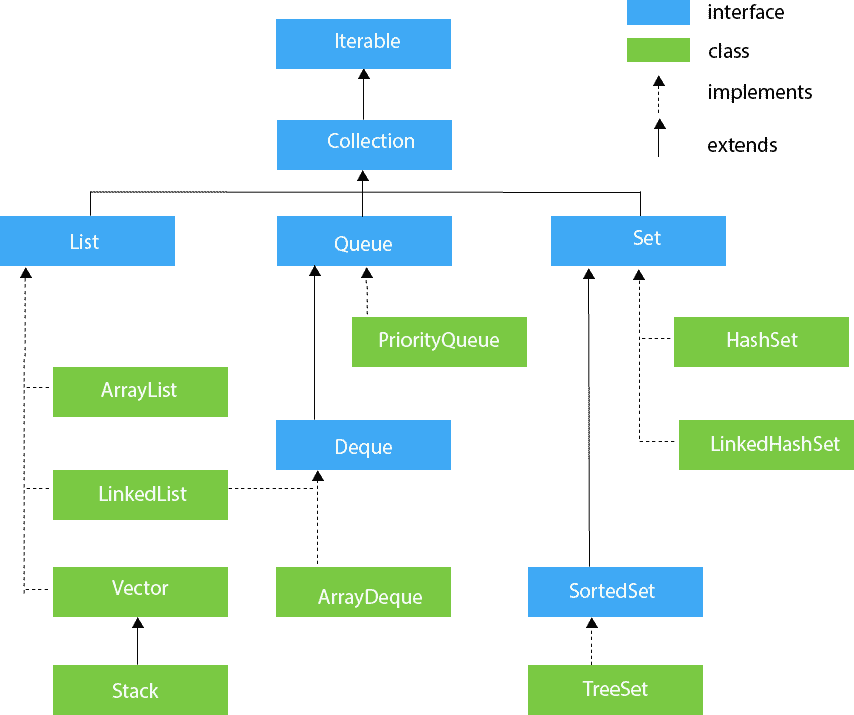
\includegraphics[width=.7\textwidth]{images/java-collection-hierarchy.png}
  \caption{Java Collections Framework hierarchy \cite{java_collection_hierarchy}.}
  \label{figure:collection_hierarchy}
\end{figure}

As shown in \hyperref[figure:collection_hierarchy]{\textbf{Figure
\ref*{figure:collection_hierarchy}}}, \texttt{Collection} is an interface that is implemented by
three different sub-interfaces, and each sub-interface is extended by different data structure
classes. Therefore, it is worth to investigate the relationship between the type of data structure
used and the output of the testing implementation.

\begin{enumerate}
  \item \texttt{List:}
  \begin{enumerate}
    \item \texttt{ArrayList}, \texttt{LinkedList}, and \texttt{Vector} implement the \texttt{List}
    interface. The main difference between them is their implementation which causes different
    performance for different operations \cite{arraylist, linkedlist, vector}.
    \item Both \texttt{Collections.sort} and \texttt{Collections.rotate} use interface over
    concrete types for the \texttt{list} parameter. This implies that both methods will only call
    methods that are defined by the \texttt{List} interface (so no \texttt{ArrayList} etc. specific
    methods).
  \end{enumerate}
  Hence, assume that \texttt{ArrayList}, \texttt{LinkedList}, and \texttt{Vector} have correct and
  complete implementation, the testing results of \texttt{Collections.sort} and
  \texttt{Collections.rotate} should not be affected by the type of data structure used.

  \item \texttt{Collection:}
  \begin{enumerate}
    \item \texttt{List}, \texttt{Queue}, and \texttt{Set} are fundamentally different from each
    other in terms of storing and manipulating the data. One crucial difference is that \texttt{Set}
    does not allow duplicate elements \cite{set}, which means that there will be certain categories
    that are not applicable when the input \texttt{coll} is a \texttt{Set}.
    \item \texttt{Collections.min} uses interface over concrete types for the \texttt{coll}
    parameter, which implies that the \texttt{min} method will only use methods that are defined by
    the \texttt{Collection} interface.
  \end{enumerate}
  Assume that \texttt{List}, \texttt{Queue}, and \texttt{Set} have been correctly and completely
  implemented, implemented, the testing results of \texttt{min} should not be affected by the type
  of data structure used as well.
\end{enumerate}

\subsubsection{Type of elements}
Another aspect to consider is the type of the elements stored in the \texttt{List} or
\texttt{Collection}. Since, all elements must be an instance of a class that implements the
\texttt{Comparable} interface \cite{comparable}, the correctness of \texttt{Collections.sort} and
\texttt{Collections.min} is then dependent on the implementation of the \texttt{compareTo} method.

In this testing assessment, the primary objective is to test the \texttt{sort}, \texttt{rotate}, and
\texttt{min} methods of the \texttt{Collections} interface. The premise for this assessment is that
all classes that implemented the \texttt{Comparable} interface have defined their respective
\texttt{compareTo} method correctly, otherwise it would have contradict with the expected output
results set for the test cases. Hence, it is assumed that the type of elements used in the testing
(e.g. \texttt{Integer}, \texttt{Double}, \texttt{Date} etc.) would not affect the test results, and
it would not be taken into consideration as one of the category partition for test inputs.

%----------------------------------------------------------------------------------------
%	List
%----------------------------------------------------------------------------------------
\subsection{Parameter: List}
\textcolor{red}{N.B.} All elements in the list must be an instance of a class that implements the
\texttt{Comparable} interface and must be mutually comparable.

\begin{category}[L]{Empty list}
  \textbf{Input:} \texttt{list = []}
  \par
  \textbf{Reason:} One of the edge cases of the \texttt{List} interface. Given this as the input,
  both \texttt{Collections.sort} and \texttt{Collections.rotate} should return an empty list as the
  output.
\end{category}

\begin{category}[L]{Single element in the list}
  \textbf{Input:} \texttt{list = [$x$]}
  \par
  \textbf{Reason:} One of the edge cases of the \texttt{List} interface. The output returned by both
  \texttt{Collections.sort} and \texttt{Collections.rotate} should be the same as the input.
\end{category}

\begin{category}[L]{More than one element in the list}
  \textbf{Input:} \texttt{list = [$x_0, x_1, \dots, x_n$]} for $n > 1$, where $n$ is the total
  number of elements in the list
  \par
  \textbf{Reason:} The is the minimum viable case for testing the actual functionality of both
  \texttt{Collections.sort} and \texttt{Collections.rotate}. This is the base form that is used to
  define other variants of the input (\textbf{Category L4 - L7}).
\end{category}

\begin{category}[L]{Repeated elements in the list}
  \textbf{Input:} \texttt{list = [$x_0, x_1, \dots, x_n$]} for $n > 1$. In addition, there exists
  some $a, b\ \text{for all } 0 \leq a,b \leq n$, the value of $x_a$ is equal to $x_b$.
  \par
  \textbf{Reason:}
  \begin{enumerate}
    \item This is to test the stability of the \texttt{Collections.sort} sorting algorithm.
  The sorting algorithm should sort the repeated elements in the same order that they appear in the
  input.
    \item This is to test that \texttt{Collections.rotate} only modifies the position of the
    elements. The value of each element should not affect the final output.
  \end{enumerate}
\end{category}

\begin{category}[L]{List contains elements of different class}
  \textbf{Input:} \texttt{list = [$x_0, x_1, \dots, x_n$]} for $n > 1$, there exists some $i, j$
  such that for all $0 \leq i,j \leq n,\  i \neq j$, the type of $x_i \neq$ type of $x_j$.
  \par
  \textbf{Reason:} This is a special category for \texttt{Collections.rotate}. Since the purpose of
  \texttt{Collections.rotate} is to modify the index of each element in the list, the actual value
  of each element should have no significant effect for the method. Therefore, the \texttt{rotate}
  method should work correspondingly when the list contains elements of different types.
\end{category}

\begin{category}[L]{List is sorted in ascending natural order of its elements}
  \textbf{Input:} \texttt{list = [$x_0, x_1, \dots, x_n$]} for $n > 1$, where the list is arranged
  according to the natural ordering \cite{java_natural_order} of its elements such that $x_k \leq
  x_{k+1}$ for all $0 \leq k \leq n$. The list can contain repeated elements.
  \par
  \textbf{Reason:} This is to test the sorting stability of \texttt{Collections.sort}. Since the
  input list is already sorted, then the elements in the output list should have the same order as
  the input list.
\end{category}

\begin{category}[L]{List is sorted in descending natural order of its elements}
  \textbf{Input:} \texttt{list = [$x_0, x_1, \dots, x_n$]} for $n > 1$, where the list is arranged
  according to the \textbf{reverse} natural ordering \cite{java_natural_order} of its elements such
  that $x_k \geq x_{k+1}$ for all $0 \leq k < n$.
  \par
  \textbf{Reason:} This is the inverse case of \textbf{Category L6}, where the input list is sorted
  in reverse order. The aim is to test the sorting stability of \texttt{Collections.sort} and also
  ensure that it can handle the cases where certain parts of the list (i.e. sub-list) are inversely
  sorted.
\end{category}

\begin{category}[L]{List size is greater than or equal to \texttt{ROTATE\_THRESHOLD}}
  \textbf{Input:} \texttt{list = [$x_0, x_1, \dots, x_n$]} for $n \geq \texttt{ROTATE\_THRESHOLD}$,
  in which the value of \\\texttt{ROTATE\_THRESHOLD} is defined as 100 in \texttt{Collections.java}
  \cite{rotate_threshold_variable}.
  \par
  \textbf{Reason:} According to the source code of \texttt{Collections.java}
  \cite{rotate_threshold_branch}, Java uses two different algorithm to rotate lists that are < or
  $\geq$ than \texttt{ROTATE\_THRESHOLD} respectively. The aim is to validate that both algorithms
  are able to correctly rotate the input list.
\end{category}

%----------------------------------------------------------------------------------------
%	distance
%----------------------------------------------------------------------------------------
\subsection{Parameter: distance}
\begin{category}[D]{Negative number}
  \textbf{Input:} \texttt{distance < 0}
  \par
  \textbf{Reason:} To ensure that the \texttt{Collections.rotate} method will work with negative
  distance input by covering the negative domain of \texttt{int} data type.
\end{category}

\begin{category}[D]{Zero}
  \textbf{Input:} \texttt{distance == 0}
  \par
  \textbf{Reason:} 0 is the default value of \texttt{int} data type in Java, and also the starting
  index value of \texttt{List}. This is to ensure that the \texttt{Collections.rotate} method will
  work when the input distance is zero.
\end{category}

\begin{category}[D]{Positive number}
  \textbf{Input:} \texttt{distance > 0}
  \par
  \textbf{Reason:} To ensure that the \texttt{Collections.rotate} method will work with positive
  distance input by covering the positive domain of \texttt{int} data type.
\end{category}

\begin{category}[D]{Larger than list size}
  \textbf{Input:} \texttt{distance > list.size()}
  \par
  \textbf{Reason:} A derivative of \textbf{Category D3}. Since the \texttt{rotate} method uses
  modulo operation on the input distance \cite{collection_rotate}, this is to test whether the
  behaviour of inputting a distance larger than \texttt{list.size()} is the same as inputting the
  value of \texttt{distance \% list.size()} \cite{collection_rotate}.
\end{category}

\begin{category}[D]{Equal to list size}
  \textbf{Input:} \texttt{distance == list.size()}
  \par
  \textbf{Reason:} This is to validate that if the distance is equal to the \texttt{list.size()},
  then \texttt{Collections.rotate} will return the the same output as the input.
\end{category}

\begin{category}[D]{Smaller than list size}
  \textbf{Input:} \texttt{distance < list.size()}
  \par
  \textbf{Reason:} A derivative of \textbf{Category D1 - D3} and the inverse case of
  \textbf{Category D4}. This is to validate the assumption that there exists some $d$ for all $d >
  \texttt{list.size()}$ and $n$ for all $n < \texttt{list.size()}$ such that \texttt{rotate(list, d)
  == rotate(list, n)}.
\end{category}

\begin{category}[D]{Equal to minimum boundary value of \texttt{int}}
  \textbf{Input:} \texttt{distance == Integer.MIN\_VALUE}
  \par
  \textbf{Reason:} The minimum value an \texttt{int} can have in Java is $-2^{31}$
  \cite{int_min_value}. The aim is to validate the assumption that if \texttt{Collections.rotate}
  works for the minimum value of \texttt{int}, then it should work correctly for any value
  \textbf{larger than the minimum value}.
\end{category}

\begin{category}[D]{Equal to maximum boundary value of \texttt{int}}
  \textbf{Input:} \texttt{distance == Integer.MAX\_VALUE}
  \par
  \textbf{Reason:} The maximum value an \texttt{int} can have in Java is $2^{31} - 1$
  \cite{int_max_value}. The aim is to validate the assumption that if \texttt{Collections.rotate}
  works for the maximum value of \texttt{int}, then it should work correctly for any value
  \textbf{smaller than the maximum value}.
\end{category}

%----------------------------------------------------------------------------------------
%	Collection
%----------------------------------------------------------------------------------------
\subsection{Parameter: Collection}
\textcolor{red}{N.B.} All elements in the collection must be an instance of a class that implements
the \texttt{Comparable} interface and must be mutually comparable.

\begin{category}[C]{Single element in collection}
  \textbf{Input:} $\texttt{coll} = \{x\}$
  \par
  \textbf{Reason:} Edge case of the \texttt{Collections.min} method. The method should only return
  the single element as the minimum element of the given collection.
\end{category}

\begin{category}[C]{More than one element in collection}
  \textbf{Input:} $\texttt{coll} = \{x_0, x_1, \dots, x_n\}\ \text{for}\ n > 1$
  \par
  \textbf{Reason:} To test whether the \texttt{Collections.min} method is able to find and return
  the minimum element of the given collection.
\end{category}

\begin{category}[C]{Repeated elements in collection}
  \textbf{Input:} $\texttt{coll} = \{x_0, x_1, \dots, x_n\}\ \text{for}\ n > 1$. In addition, there
  exists some $a, b\ \text{for all } 0 \leq a,b \leq n,\  a \neq b$, the value of $x_a$ is equal to
  $x_b$.
  \par
  \textbf{Reason:} To test whether the \texttt{Collections.min} method is able to handle repeated
  elements and correctly return the minimum element of the given collection.
\end{category}

\begin{category}[C]{Repeated minimum elements in collection}
  \textbf{Input:} $\texttt{coll} = \{x_0, x_1, \dots, x_n\}\ \text{for}\ n > 1$. In addition, there
  exists some $a, b\ \text{for all } 0 \leq a,b \leq n,\  a \neq b$, the value of $x_a$ is equal to
  $x_b$ and both $x_a$ and $x_b$ are the minimum elements in the collection.
  \par
  \textbf{Reason:} A derivative of \textbf{Category C3} to test the stability of
  \texttt{Collections.min} method. It is expected that the method will treat the repeated minimum
  elements as the same element and return correctly.
\end{category}

\begin{category}[C]{Collection contains the minimum possible value of the class}
  \textbf{Input:} $\texttt{coll} = \{x_0, x_1, \dots, x_n\}\ \text{for}\ n > 1$, and there exists a
  $k$ where $0 \leq k \leq n$ such that $x_k$ is the minimum possible value of the element's class.
  \par
  \textbf{Reason:} To cover the boundary case of \texttt{Collections.min}, and to test whether the
  method always return the minimum possible value of the class when the given collection contains
  it.
\end{category}

\begin{category}[C]{Collection is in ascending natural order of its elements}
  \textbf{Input:} $\texttt{coll} = \{x_0, x_1, \dots, x_n\}\ \text{for}\ n > 1$, where the
  collection is arranged according to the natural ordering \cite{java_natural_order} of its elements
  such that $x_k \leq x_{k+1}$ for all $0 \leq k \leq n$. The collection can contain repeated
  elements.
  \par
  \textbf{Reason:} Since the given collection is already sorted, then the minimum element returned
  should have the same value as first element of the collection.
\end{category}

\begin{category}[C]{Collection is in descending natural order of its elements}
  \textbf{Input:} $\texttt{coll} = \{x_0, x_1, \dots, x_n\}\ \text{for}\ n > 1$, where the
  collection is arranged according to the natural ordering \cite{java_natural_order} of its elements
  such that $x_k \geq x_{k+1}$ for all $0 \leq k < n$. The collection can contain repeated elements.
  \par
  \textbf{Reason:} The inverse case of \textbf{Category C6}. Since, the given collection is sorted
  in reverse order, then the minimum element returned should have the same value as the last element
  of the collection.
\end{category}

%----------------------------------------------------------------------------------------
%	Test cases
%----------------------------------------------------------------------------------------
\section{Test Cases}
\subsection{\texttt{Collections.sort(List<T> list)}}
\begin{enumerate}
  \item \textbf{Test Case 1}
  \par\quad\textbf{Categories:} L2

  \par\quad\textbf{Input:} \texttt{list = [1]}

  \item \textbf{Test Case 2}
  \par\quad\textbf{Categories:} L3 $\wedge$ L4

  \par\quad\textbf{Input:} \texttt{list = [6, 8, 2, 4, 7, 5, 3, 2, 9]}

  \item \textbf{Test Case 3}
  \par\quad\textbf{Categories:} L3 $\wedge$ L7
  \par\quad\textbf{Input:} \texttt{list = [9, 8, 7, 6, 5, 4, 3, 2, 1]}
\end{enumerate}

\subsection{\texttt{Collections.rotate(List<?> list, int distance)}}
\begin{enumerate}
  \item \textbf{Test Case 1}
  \par\quad\textbf{Categories:} L1, D2 $\wedge$ D5
  \par\quad\textbf{Input:} \texttt{list = [], distance = 0}

  \item \textbf{Test Case 2}
  \par\quad\textbf{Categories:} L3 $\wedge$ L5, D3 $\wedge$ D4 $\wedge$ D8
  \par\quad\textbf{Input:} \texttt{list = [1, 2, `a', `b', 3.7, 4, "str"], distance = $2^{31} - 1$}

  \item \textbf{Test Case 3}
  \par\quad\textbf{Categories:} L3 $\wedge$ L8, D1 $\wedge$ D6 $\wedge$ D7
  \par\quad\textbf{Input:} \texttt{list = [1, 2, $\dots$, 200, 201], distance = $2^{31} - 1$}
\end{enumerate}

\subsection{\texttt{Collections.min(Collection<? extends T> coll)}}
\begin{enumerate}
  \item \textbf{Test Case 1}
  \par\quad\textbf{Categories:} C1
  \par\quad\textbf{Input:} $\texttt{coll} = \{\texttt{1}\}$

  \item \textbf{Test Case 2}
  \par\quad\textbf{Categories:} C2 $\wedge$ C7
  \par\quad\textbf{Input:} $\texttt{coll} = \{\texttt{1, 2, 3, 4, 5, 6, 7, 8, 9}\}$

  \item \textbf{Test Case 3}
  \par\quad\textbf{Categories:} C2 $\wedge$ C3 $\wedge$ C4 $\wedge$ C5

  \par\quad\textbf{Input:} $\texttt{coll} = \{\texttt{6, 8, 2, 4, 7, Integer.MIN\_VALUE, 5, 3, 2,
  9}\}$
\end{enumerate}

%----------------------------------------------------------------------------------------
%	Metamorphic relation
%----------------------------------------------------------------------------------------
\section{Metamorphic Relations}
\subsection{\texttt{Collections.sort(List<T> list)}}
The return type of \texttt{Collections.sort} is \texttt{void} \cite{collection_sort}, the input list
is modified when the method is called.

\begin{lstlisting}[language = Java, frame = trBL, firstnumber = last, escapeinside={(*@}{@*)}]
List x = new ArrayList<>(Arrays.asList((*@$x_0, x_1, \dots, x_n$@*)));
List xTransformed = new ArrayList<>(x); // defined as x' below

(*@$\dots$@*) // see input transformation below

// x and xTransformed are modified directly after method call
Collections.sort(x);
Collections.sort(xTransformed);
\end{lstlisting}

\begin{table}[H]
  \centering
  \begin{tabular}{p{3.85cm}|l|c}
  \hline
  \multicolumn{1}{c|}{\textbf{Description}} & \multicolumn{1}{c|}{\textbf{Input Transformation}} &
  \textbf{Relation} \\ \hline
  Reverse the original input list & \texttt{Collections.reverse(x')} & \texttt{x'.equals(x)} \\ \hline
  Double the size and content of original input by adding itself & \texttt{x'.addAll(x);} &
  \adjustbox{valign=t}{\makecell{\texttt{x'.size() == 2 * x.size, } \\ \texttt{x'[2n] == x[n], } \\
  \texttt{x'[2n+1] == x[n]}}} \\ \hline
  \end{tabular}
\end{table}

\subsection{\texttt{Collections.rotate(List<?> list, int distance)}}
The return type of \texttt{Collections.rotate} is \texttt{void} \cite{collection_rotate}, the input
list is modified when the method is called.

\begin{lstlisting}[language = Java, frame = trBL, escapeinside={(*@}{@*)}]
List x = new ArrayList<>(Arrays.asList((*@$x_0, x_1, \dots, x_n$@*)));
int d = ...;

List xTransformed = new ArrayList<>(x); // defined as x' below
int dTransformed = ...; // defined as d' below

(*@$\dots$@*) // see input transformation below

// x and xTransformed are modified directly after method call
Collections.rotate(x, d);
Collections.rotate(xTransformed, dTransformed);
\end{lstlisting}

\begin{table}[H]
  \centering
  \begin{tabular}{p{3.85cm}|l|c}
  \hline
  \multicolumn{1}{c|}{\textbf{Description}} & \multicolumn{1}{c|}{\textbf{Input Transformation}} &
  \textbf{Relation} \\ \hline
  Reverse the original input list, convert distance to opposite sign &
  \adjustbox{valign=t}{\makecell{\texttt{Collections.reverse(x')} \\ \texttt{dTransformed = -d}}}  &
  \adjustbox{valign=t}{\makecell{After reversing \texttt{x'} again,\\ \texttt{x'.equals(x)}}} \\
  \hline
  Add the value of \texttt{d * x.size()} to distance &
  \adjustbox{valign=t}{\makecell{\texttt{dTransformed = }\\\texttt{d * (1 + x.size())}}} &
  \texttt{x'.equals(x)} \\
  \hline
  \end{tabular}
\end{table}

\subsection{\texttt{Collections.min(Collection<? extends T> coll)}}
The return type of \texttt{Collections.min} is type of the elements in the list
\cite{collection_min}.

\begin{lstlisting}[language = Java, frame = trBL, escapeinside={(*@}{@*)}]
List x = new ArrayList<>(Arrays.asList((*@$x_0, x_1, \dots, x_n$@*)));
List xTransformed = new ArrayList<>(x); // defined as x' below

(*@$\dots$@*) // see input transformation below

// <T> is a placeholder for the type of elements in the list
<T> z = Collections.min(x);
<T> zTransformed = Collections.min(xTransformed);
\end{lstlisting}

\begin{table}[H]
  \centering
  \begin{tabular}{p{8cm}|l|c}
  \hline
  \multicolumn{1}{c|}{\textbf{Description}} & \multicolumn{1}{c|}{\textbf{Input Transformation}} &
  \textbf{Relation} \\ \hline
  Add an element smaller than the minimum element in the original collection & \texttt{x'.add($x$)}
  & \texttt{z' < z} \\ \hline
  Add an element greater than the minimum element in the original collection & \texttt{x'.add($x$)} &
  \texttt{z' == z} \\ \hline
  \hline
  \end{tabular}
\end{table}

\textcolor{red}{N.B.} For the first relation, if the minimum element in the original collection is
already the minimum possible elements for the class, then the new element added is equal to the
minimum element in the original collection. The relation will then be \texttt{z' == z}.

%----------------------------------------------------------------------------------------
%	Remarks
%----------------------------------------------------------------------------------------
\section{Remarks}


\printbibliography

\end{document}
